\section{Control Flow Graph}\todo{Update so it fits to the impl.}
The \texttt{cfg} module contains a class, \texttt{CFG}, that takes an AST and builds a CFG from it.
The CFG is built by traversing the generated AST using the visitor pattern.\cite{design_patterns}
The visitor pattern is implemented by the AST module, and our CFG module utilizes this implementation.

\begin{figure}[H]
  \begin{subfigure}[b]{0.2\textwidth}
    \begin{lstlisting}[style=python]
if True:
    x = 0
elif False:
    y = 0
else:
    z = 0
    \end{lstlisting}
    \caption{Code example}
    \label{CFG_if_code}
  \end{subfigure}
  ~~~ %add desired spacing between images, e. g. ~, \quad, \qquad, \hfill etc. 
  %(or a blank line to force the subfigure onto a new line)
  \begin{subfigure}[b]{0.4\textwidth}
    \begin{lstlisting}[style=default, basicstyle=\footnotesize, numbers=none]
If
   test
      NameConstant
   body
      [Assign]
   orelse
      If
         test
            NameConstant
         body
            [Assign]
         orelse
            [Assign]
    \end{lstlisting}
    \caption{Abstract Syntax Tree}
    \label{CFG_if_ast}
  \end{subfigure}
  ~
  \begin{subfigure}[b]{0.3\textwidth}
    \centering
    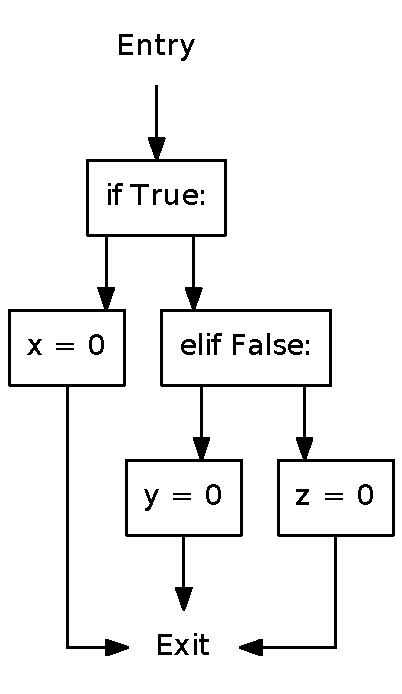
\includegraphics[scale=.5]{./figures/if_else_elif.pdf}
    \caption{Possible flows}
    \label{CFG_if_flow}
  \end{subfigure}

  \caption{An AST and the expected CFG}
  \label{CFG_if_else}  
\end{figure}

\subsection{From AST to CFG}
Implementing the CFG requires considering all the cases mentioned in \cref{python:control_structures}.
\Cref{CFG_if_else} shows an one of the cases with the intermediate AST step included (\cref{CFG_if_ast}).
Here the AST is visualised as a tree, where the first node is an \texttt{If} node \footnote{An AST for a complete program starts with a \texttt{Module} node, but this is not shown here in order to simplify the tree}
This node contains a test node, a body, represented as a list of nodes, and an orelse body, also represented as a list of nodes.
In this example the conditions are \texttt{NameConstant} nodes and all statements are \texttt{Assign} nodes.
The orelse body of the outer \texttt{If} node contains another \texttt{If} node which contains the \texttt{elif} which has the else in its orelse body.

The CFG of the program is generated by traversing the AST and creating a CFG node at each node.
These nodes are then connected so the resulting CFG reflects the flow of the program.
The implementation of the \texttt{If} visitor will be described in the following.

\subsection{Visitor implementation}
\Cref{visit_if_code} shows the implementation of visiting an \texttt{If} AST node.
First, another visitor, the \texttt{LabelVisitor} is used to find labels of statements in the CFG.
In \cref{if_test_label} it is used to generate the label of the condition in the \texttt{if}.
Afterwards a CFG node is created for the condition and appended to the list of CFG nodes.
In \cref{if_body_handling} the body of the \texttt{if} is handled by the \texttt{stmt\_star\_handler} method.
This method visits all nodes in the body and connects them properly.
\Cref{if_orelse_handling} now handles \texttt{elif} and \texttt{else} cases.
Again \texttt{stmt\_star\_handler} handles the connection of the bodies.

Through the implementation a number of 'last nodes' are being kept track of.
This is for instance seen in \cref{if_last_statements} where the 'last nodes' of the orelse node are added to the 'last nodes' of the body.
A 'last statement' is in this context any statement that needs to be connected to the subsequent statement of the \texttt{if}.
Among these are \texttt{raise} statements, \texttt{return} statements and the last statements of the body, \texttt{elif} bodies and the \texttt{else} body. \todo{måske bedre eksempler og tegninger med pile}
These are sent to the calling function by returning a \texttt{ControlFlowNode} in \cref{if_return}.
This calling function is \texttt{stmt\_star\_handler} which, as stated above, connects all the nodes properly.

\begin{lstlisting}[style=python, caption={Visiting an If AST node.}, label={visit_if_code}, escapeinside={(*@}{@*)}, breaklines=true]
def visit_If(self, node):
    label_visitor = LabelVisitor() (*@\label{if_test_label}@*)
    label_visitor.visit(node.test)

    test = self.append_node(Node(label_visitor.result, node, line_number = node.lineno))
    self.add_if_label(test)

    body_connect_stmts = self.stmt_star_handler(node.body) (*@ \label{if_body_handling} @*)
    test.connect(body_connect_stmts.first_statement)
        
    if node.orelse: (*@ \label{if_orelse_handling} @*)
        orelse_last_nodes = self.handle_or_else(node.orelse, test)
        body_connect_stmts.last_statements.extend(orelse_last_nodes) (*@ \label{if_last_statements} @*)
    else:
        body_connect_stmts.last_statements.append(test)

    last_statements = self.remove_breaks(body_connect_stmts.last_statements)

    return ControlFlowNode(test, last_statements, break_statements=body_connect_stmts.break_statements) (*@ \label{if_return} @*)
\end{lstlisting}
